% Graphic for TeX using PGF
% Title: /home/lihram/git/github.com/lihram/matrix-aau/report/graphics/design_constraints.dia
% Creator: Dia v0.97+git
% CreationDate: Sat May 16 12:44:00 2020
% For: lihram
% \usepackage{tikz}
% The following commands are not supported in PSTricks at present
% We define them conditionally, so when they are implemented,
% this pgf file will use them.
\ifx\du\undefined
  \newlength{\du}
\fi
\setlength{\du}{15\unitlength}
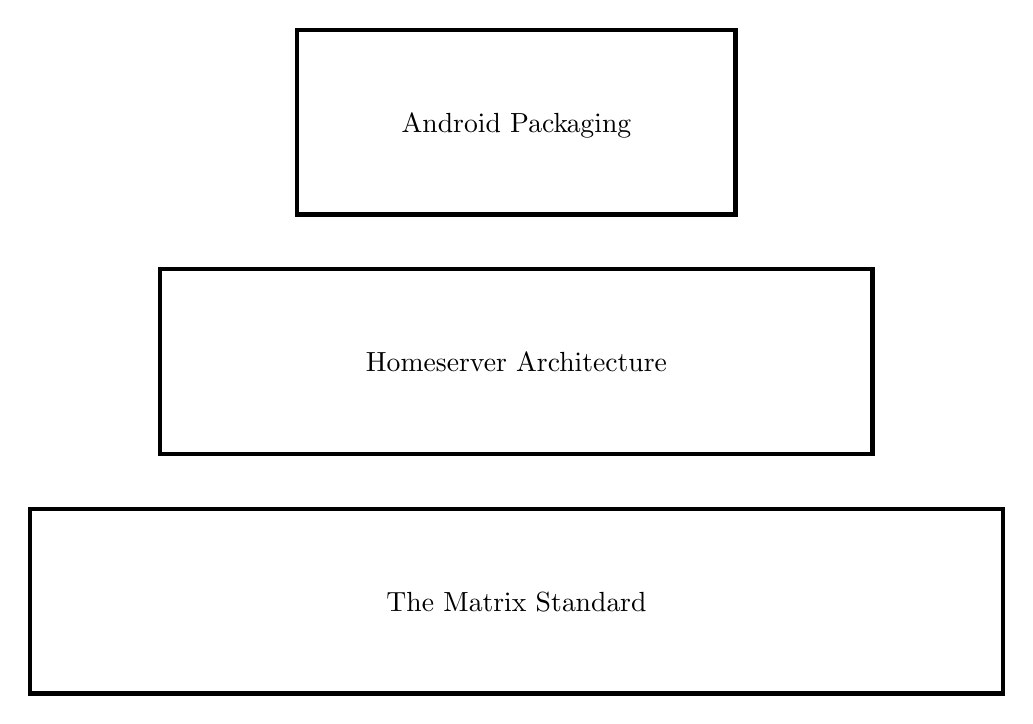
\begin{tikzpicture}[even odd rule]
\pgftransformxscale{1.000000}
\pgftransformyscale{-1.000000}
\definecolor{dialinecolor}{rgb}{0.000000, 0.000000, 0.000000}
\pgfsetstrokecolor{dialinecolor}
\pgfsetstrokeopacity{1.000000}
\definecolor{diafillcolor}{rgb}{1.000000, 1.000000, 1.000000}
\pgfsetfillcolor{diafillcolor}
\pgfsetfillopacity{1.000000}
\pgfsetlinewidth{0.100000\du}
\pgfsetdash{}{0pt}
\pgfsetmiterjoin
{\pgfsetcornersarced{\pgfpoint{0.000000\du}{0.000000\du}}\definecolor{diafillcolor}{rgb}{1.000000, 1.000000, 1.000000}
\pgfsetfillcolor{diafillcolor}
\pgfsetfillopacity{1.000000}
\fill (10.198750\du,18.700000\du)--(10.198750\du,23.150000\du)--(33.648750\du,23.150000\du)--(33.648750\du,18.700000\du)--cycle;
}{\pgfsetcornersarced{\pgfpoint{0.000000\du}{0.000000\du}}\definecolor{dialinecolor}{rgb}{0.000000, 0.000000, 0.000000}
\pgfsetstrokecolor{dialinecolor}
\pgfsetstrokeopacity{1.000000}
\draw (10.198750\du,18.700000\du)--(10.198750\du,23.150000\du)--(33.648750\du,23.150000\du)--(33.648750\du,18.700000\du)--cycle;
}% setfont left to latex
\definecolor{dialinecolor}{rgb}{0.000000, 0.000000, 0.000000}
\pgfsetstrokecolor{dialinecolor}
\pgfsetstrokeopacity{1.000000}
\definecolor{diafillcolor}{rgb}{0.000000, 0.000000, 0.000000}
\pgfsetfillcolor{diafillcolor}
\pgfsetfillopacity{1.000000}
\node[anchor=base,inner sep=0pt, outer sep=0pt,color=dialinecolor] at (21.923750\du,21.169966\du){The Matrix Standard};
\pgfsetlinewidth{0.100000\du}
\pgfsetdash{}{0pt}
\pgfsetmiterjoin
{\pgfsetcornersarced{\pgfpoint{0.000000\du}{0.000000\du}}\definecolor{diafillcolor}{rgb}{1.000000, 1.000000, 1.000000}
\pgfsetfillcolor{diafillcolor}
\pgfsetfillopacity{1.000000}
\fill (13.346250\du,12.930000\du)--(13.346250\du,17.380000\du)--(30.501250\du,17.380000\du)--(30.501250\du,12.930000\du)--cycle;
}{\pgfsetcornersarced{\pgfpoint{0.000000\du}{0.000000\du}}\definecolor{dialinecolor}{rgb}{0.000000, 0.000000, 0.000000}
\pgfsetstrokecolor{dialinecolor}
\pgfsetstrokeopacity{1.000000}
\draw (13.346250\du,12.930000\du)--(13.346250\du,17.380000\du)--(30.501250\du,17.380000\du)--(30.501250\du,12.930000\du)--cycle;
}% setfont left to latex
\definecolor{dialinecolor}{rgb}{0.000000, 0.000000, 0.000000}
\pgfsetstrokecolor{dialinecolor}
\pgfsetstrokeopacity{1.000000}
\definecolor{diafillcolor}{rgb}{0.000000, 0.000000, 0.000000}
\pgfsetfillcolor{diafillcolor}
\pgfsetfillopacity{1.000000}
\node[anchor=base,inner sep=0pt, outer sep=0pt,color=dialinecolor] at (21.923750\du,15.399966\du){Homeserver Architecture};
\pgfsetlinewidth{0.100000\du}
\pgfsetdash{}{0pt}
\pgfsetmiterjoin
{\pgfsetcornersarced{\pgfpoint{0.000000\du}{0.000000\du}}\definecolor{diafillcolor}{rgb}{1.000000, 1.000000, 1.000000}
\pgfsetfillcolor{diafillcolor}
\pgfsetfillopacity{1.000000}
\fill (16.646250\du,7.160000\du)--(16.646250\du,11.610000\du)--(27.201250\du,11.610000\du)--(27.201250\du,7.160000\du)--cycle;
}{\pgfsetcornersarced{\pgfpoint{0.000000\du}{0.000000\du}}\definecolor{dialinecolor}{rgb}{0.000000, 0.000000, 0.000000}
\pgfsetstrokecolor{dialinecolor}
\pgfsetstrokeopacity{1.000000}
\draw (16.646250\du,7.160000\du)--(16.646250\du,11.610000\du)--(27.201250\du,11.610000\du)--(27.201250\du,7.160000\du)--cycle;
}% setfont left to latex
\definecolor{dialinecolor}{rgb}{0.000000, 0.000000, 0.000000}
\pgfsetstrokecolor{dialinecolor}
\pgfsetstrokeopacity{1.000000}
\definecolor{diafillcolor}{rgb}{0.000000, 0.000000, 0.000000}
\pgfsetfillcolor{diafillcolor}
\pgfsetfillopacity{1.000000}
\node[anchor=base,inner sep=0pt, outer sep=0pt,color=dialinecolor] at (21.923750\du,9.629966\du){Android Packaging};
\end{tikzpicture}
